\documentclass[10pt,a4paper]{ctexart}

% Compile with XeLaTeX. Compact three-column layout.
\usepackage[a4paper,margin=0.30in,includeheadfoot]{geometry}
\usepackage{amsmath,amssymb,mathtools}
\usepackage{siunitx}
\usepackage{multicol}
\usepackage{booktabs,tabularx,array}
\usepackage{enumitem}
\usepackage{titlesec}
\usepackage{xcolor}
\usepackage{microtype}
\usepackage{fancyhdr}
\usepackage[hidelinks]{hyperref}

\pagestyle{fancy}
\fancyhf{}
\fancyfoot[C]{\small\thepage}
\setlength{\headheight}{5pt}
\setlength{\headsep}{2pt}
\setlength{\footskip}{12pt}
\setlength{\columnsep}{0.14in}
\setlength{\columnseprule}{0.2pt}
\setlength{\parindent}{0pt}
\setlength{\parskip}{0.5pt}
\linespread{0.91}
\emergencystretch=2em
\AtBeginDocument{\fontsize{10pt}{9.1pt}\selectfont}

\titleformat{\section}{\normalsize\bfseries\color{blue!55!black}}{}{0pt}{}
\titlespacing*{\section}{0pt}{2pt}{0.5pt}
\titleformat{\subsection}{\normalsize\bfseries\color{black!75}}{}{0pt}{}
\titlespacing*{\subsection}{0pt}{1.5pt}{0pt}
\titleformat{\subsubsection}{\small\bfseries}{}{0pt}{}
\titlespacing*{\subsubsection}{0pt}{1pt}{0pt}
\setlist{nosep,leftmargin=*,topsep=0.5pt,partopsep=0pt}
\setlist[itemize]{label=\textbullet}
\setlist[enumerate]{label=\arabic*.,labelsep=0.3em}

\newcommand{\key}[1]{\textbf{#1}}
\newcommand{\formula}[1]{%
  \par\vspace{1pt}\begingroup
  \setlength{\abovedisplayskip}{0pt}\setlength{\belowdisplayskip}{0pt}
  \[#1\]\endgroup\vspace{1pt}}
\newcolumntype{Y}{>{\raggedright\arraybackslash}X}

\begin{document}
\begin{multicols*}{3}
\sloppy

\section{1. Introduction \& Integration}
\subsection{What is flexible bioelectronics}
\begin{itemize}
  \item \key{Electronics:} physics, engineering, technology and applications
  dealing with the emission, flow and control of electrons in vacuum and matter.
  \item \key{Flexible electronics:} the production of electronic components fabricated on a
  flexible substrate (typically polymer), giving thinner, lighter, softer,
  conformal and potentially stretchable systems.
  \item Main course goal: integrate high-performance electronics with soft,
  dynamic and biologically compatible interfaces for on-patient monitoring,
  diagnosis, therapy and human--machine interaction.
\end{itemize}

\subsection{Electronic categories}
\begin{itemize}
  \item Digital, analogue, microelectronics, integrated circuits (ICs),
  power electronics, optoelectronics, semiconductor devices and embedded systems.
  \item \key{Discrete circuit:} individually packaged components; customizable
  but bulky and costly at high volume.
  \item \key{Monolithic circuit:} devices fabricated on one substrate; high
  density, low unit cost at volume, but requires cleanroom processing and is
  fixed after design.
\end{itemize}

\subsection{Integration and Moore's law}
\begin{itemize}
  \item Integration evolved from vacuum tubes to transistors, ICs and
  nanoscale CMOS; resistor, capacitor, diode and transistor can be made in
  compatible semiconductor processes.
  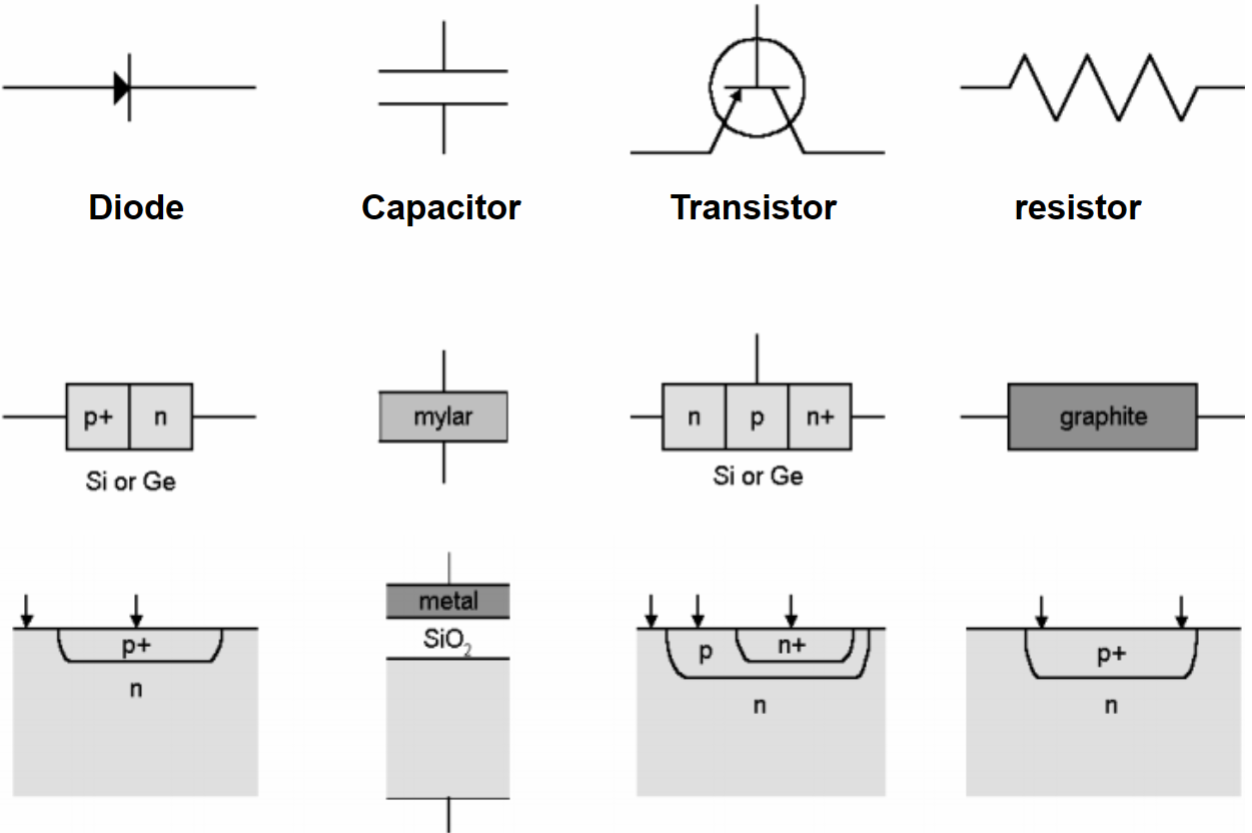
\includegraphics[width=1\linewidth]{BasicComponents.png}
  \item \key{Moore's law:} transistor count in a dense IC approximately
  doubles every two years (an observation/trend, not a physical law).
  \item Scaling improves switching speed, energy use and miniaturization,
  but introduces purity, heat, fabrication and mass-production challenges.
\end{itemize}

\subsection{Why flexible bioelectronics}
\begin{itemize}
  \item \key{Manufacturing cost:} Modern intel fabrication capital cost > 3,000,000,000.00 USD, 
  while modest flex electronics fabrication capital cost < 3,000,000.00 USD
  \item \key{Market:} enables embedding simple intelligence with cost-efficient manufacturing techniques 
  \item Conventional devices are hard/planar; organs and skin are soft,
  curved, moving and hydrated. Rigid interfaces cause discomfort, poor
  contact, motion artefact and low-fidelity signals.
  \item \key{Healthcare challenges:} centralized, slow, invasive, expensive,
  expertise-dependent testing and delayed diagnosis.
  \item \key{Desired properties:} conformality, flexibility/stretchability,
  stable adhesion, breathability, biocompatibility, low power and wireless
  communication.
  \item \key{Key design principle:} preserve high-performance active materials
  while reducing effective stiffness by thinning, patterning or embedding
  them in soft substrates.
\end{itemize}

\subsection{Cross of biology and devices}
\begin{itemize}
  \item Biology | Interface | Device
  \item Interface needs: High performance, flexible, high though-put
\end{itemize}

\subsection{E.g. Bio-Compatible Soft ECoG}
\begin{itemize}
  \item \key{Currently:} with wires, monitored by bulky medical equipment
  \item \key{Future:} wireless, monitored by portable interfaces, such as smartphones
\end{itemize}

\subsection{E.g. Complex 3D Structures manufacturing}
\begin{itemize}
  \item \key{Method:} Stress-Induced Folding, Two-Photon Lithography, 
  Direct-Writing Printing, 3D Photopatterning
  \item Can we exploit today’s the most advanced manufacturing technologies in semiconductor industry? \\
  -Yes, but selectively. Today’s advanced semiconductor manufacturing—EUV lithography, 
  atomic-layer deposition, nanoscale etching, and heterogeneous integration—can be exploited, 
  but access is limited by cost, equipment, materials, yield, and specialized expertise.
  \item Can we nano/microfab electronics from the existing highest-performance electronic materials 
  and then transform them into 3D devices?\\
  -Yes, in principle. High-performance materials can be nano/microfabricated and integrated into 3D devices using stacking, 
  transfer printing, folding, origami/kirigami, molding, and additive fabrication. 
  However, preserving electrical performance during deformation, ensuring reliable interconnects, heat dissipation, 
  and scalable manufacturing remain major challenges.
\end{itemize}


\section{2. Devices \& Materials}
\subsection{Band theory}
\begin{itemize}
  \item Atomic orbitals broaden into energy bands: valence band (VB),
  conduction band (CB), separated by band gap $E_g$.
  \item \key{Fermi level}: energy with maximum electron occupation
  probability at absolute zero.
  \item Metals: overlapping bands or $E_g\approx0$; semiconductors: moderate
  gap; insulators: large gap. Examples:
  Si $E_g=1.12$ eV, Ge $=0.66$ eV, GaAs $=1.41$ eV,
  SiO$_2\approx9$ eV, diamond $=5.47$ eV.
  \item Donors (N, P, As) produce \key{n-type}; acceptors (B, Al, Ga)
  produce \key{p-type} material.
\end{itemize}

\subsection{Electronic building blocks}
\begin{itemize}
  \item \key{Resistor/capacitor}: circuit elements and pressure, strain,
  temperature, gas and photodetectors.
  \item \key{Diode}: rectification; also LED, photodetector and solar cell.
  Emission color is set by semiconductor band gap.
  \item \key{Transistor}: switch, amplifier, sensor and ion-to-electron
  converter; important for amplifying weak biological signals.
\end{itemize}
\formula{\displaystyle
\mu_{\rm lin}=\frac{L}{WC_iV_D}\frac{\partial I_D}{\partial V_G}
\ (V_D\ll V_G),\qquad
\mu_{\rm sat}=\frac{2L}{WC_i}\frac{\partial I_D}{\partial V_G}
\ (V_D\ge V_G)}

\subsection{Crystal and material classes}
\begin{itemize}
  \item Si has diamond lattice; common structures include FCC, BCC and HCP.
  Miller notation: $[abc]$ direction, $(abc)$ plane; crystal orientation
  affects wafer processing and anisotropic etching.
  \item Single crystal: long-range order and high electronic performance.
  Polycrystal: grain boundaries affect transport. Amorphous materials have
  lower thermal conductivity, can be transparent and stable, but deform more.
  \item Candidate materials: Si, III--V (GaAs), metal oxides, polymers,
  small molecules, graphene and carbon nanotubes.
\end{itemize}

\subsection{Soft and emerging materials}
\begin{itemize}
  \item Conventional electronics fail at only about $1$--$3\%$ strain;
  skin reaches $\sim30\%$ and joints can reach $\sim100\%$.
  \item Soft substrates: PDMS, polyurethane, hydrogels and composites;
  matching Young's modulus to tissue reduces mismatch and irritation.
  \item \key{Liquid metals}: Ga, EGaIn (75.2\% Ga/24.8\% In) and Galinstan.
  They remain conductive while deforming (up to about 700\% strain).
  Ga alloys form an oxide skin in oxygen; injection/vacuum filling patterns
  them into microchannels.
  \item \key{2D materials}: graphene, black phosphorus and MXene.
  Single/few atomic layers give high surface area, conductivity,
  transparency, flexibility and easy functionalization.
\end{itemize}

\section{3. Mechanics \& Design}
\subsection{Conformability}
\begin{itemize}
  \item Conformality is the ability to maintain intimate contact with
  rough, curved skin. Thickness dominates: thinner layers bend more easily
  and follow topography better.
\end{itemize}
\formula{\displaystyle
D=\frac{Et^3}{12(1-\nu^2)}}
\begin{itemize}
  \item $D$: bending stiffness; $E$: Young's modulus; $t$: thickness;
  $\nu$: Poisson ratio. The cubic $t^3$ dependence means a small thickness
  reduction greatly lowers stiffness.
  \item Engineer low $E$ and low $t$, while retaining electrical and
  mechanical reliability.
\end{itemize}

\subsection{Stretchable layouts}
\begin{itemize}
  \item \key{Wavy/wrinkled}: prestrain a soft substrate, attach a stiff thin
  film, then release; out-of-plane waves accommodate extension.
  \item \key{Serpentine}: meandering ribbons rotate, bend and buckle so
  material strain is much lower than applied strain. Important parameters:
  width $w$, arc radius $R$, arc angle $\alpha$, arm length $l$.
  Smaller $w/R$ and longer arms generally improve stretchability.
  \item \key{Island--bridge}: rigid functional islands connected by soft,
  wavy or serpentine bridges. Non-coplanar layouts are usually more
  stretchable; fractal interconnects increase coverage and compliance.
  \item Origami/kirigami and composite structures add geometric
  deformation, fatigue resistance and mechanical buffering.
\end{itemize}

\subsection{Interface requirements}
\begin{itemize}
  \item \key{Adhesion}: must be strong, conformal and durable under motion,
  sweat and repeated loading. Dry adhesion uses van der Waals, electrostatic,
  friction or mechanical interlocking; wet adhesion uses capillary,
  hydrogen-bonding, viscous and chemical interactions.
  \item \key{Breathability}: permits air/moisture exchange and reduces sweat
  accumulation. \key{Biocompatibility}: no toxicity, irritation, allergy or
  disruption of tissue function. \key{Biodegradability}: safe dissolution
  can avoid retrieval surgery and persistent waste.
\end{itemize}

\section{4. Biomarkers \& Wearable Sensing}
\subsection{Biofluids}
\begin{center}\small
\begin{tabularx}{\linewidth}{@{}lYY@{}}
\toprule
Fluid & Advantages & Main limitations\\
\midrule
Sweat & Non-invasive; surface-accessible; electrolytes/metabolites/hormones
& low volume, evaporation, contamination, rate and site variation\\
ISF & Close to blood for small molecules; rich biomarkers
& invasive sampling, low volume, discomfort\\
Tears & Continuous, non-invasive secretion
& very low volume; eye engineering; weak blood correlation\\
Saliva & Non-invasive, continuously available, large daily volume
& viscosity; food/drink contamination; production varies\\
Urine & Rich and abundant biomarker source
& wearable use limited to urination events\\
\bottomrule
\end{tabularx}
\end{center}

\subsection{Biomarker classes}
\begin{itemize}
  \item \key{Electrolytes}: Na$^+$, K$^+$, Mg$^{2+}$, Ca$^{2+}$, Cl$^-$;
  hydration, cardiac, liver and metabolic status.
  \item \key{Metabolites}: glucose, lactate, uric acid, alcohol and amino
  acids; diabetes, metabolism and exercise. Sweat glucose is typically
  10--100 times lower than blood glucose.
  \item \key{Hormones}: cortisol, estradiol and peptides; stress,
  endocrine, reproductive, sleep and mood monitoring.
  \item Proteins/enzymes (cytokines, troponin, LDH), nucleic acids,
  bacteria/cells, drugs and other small molecules support cardiovascular,
  cancer, wound, infection and therapeutic monitoring.
\end{itemize}

\subsection{Recognition and transduction}
\begin{itemize}
  \item Biorecognition elements: enzymes, antibodies/affinity proteins,
  peptides, aptamers, receptors and molecularly imprinted polymers (MIPs).
  They bind/catalyse the target and are immobilized on a transducer.
  \item Enzyme example: glucose oxidase catalyses glucose, producing H$_2$O$_2$;
  electrode redox current increases with analyte concentration.
  \item Aptamer: synthetic ssDNA/RNA binds target; target-induced
  conformational change changes current, voltage, impedance, fluorescence
  or color. Modes include sandwich, dissociation, competitive replacement
  and structure switching.
\end{itemize}

\begin{center}\small
\begin{tabularx}{\linewidth}{@{}lY@{}}
\toprule
Method & Principle / typical use\\
\midrule
Amperometric & redox current $\propto$ concentration; glucose/lactate\\
Potentiometric & equilibrium potential; ion-selective sensing\\
Voltammetric & current versus applied potential; electroactive species\\
Impedimetric & binding changes AC impedance\\
Optical & absorption, reflection, fluorescence or color\\
Electromechanical & pressure, strain, bending, acceleration or vibration\\
\bottomrule
\end{tabularx}
\end{center}

\section{5. Processing I: Cleanroom \& Lithography}
\subsection{Safety and contamination}
\begin{itemize}
  \item Identify chemical, electrical, fire and sharps hazards; use PPE,
  correct containers, exits/showers and MSDS. HF is a contact poison and
  attacks glass; never treat it as an ordinary acid.
  \item Cleanroom defects include particles, organics, ions, moisture and
  surface damage. DI water is ion-free: at $25^\circ$C,
  $[H^+][OH^-]=10^{-14}$, $[H^+]=[OH^-]=10^{-7}$ and
  resistivity $\approx18.5~\mathrm{M\Omega\,cm}$.
\end{itemize}

\subsection{Wafer cleaning}
\begin{enumerate}
  \item DI-water ultrasonic/megasonic clean removes particles and soluble ions.
  \item RCA SC-1: DI:H$_4$NOH:H$_2$O$_2=5:1:1$, typically
  $75$--$80^\circ$C for 10 min; organic/particle clean, forms $\sim1$ nm SiO$_2$.
  \item Optional HF 1:50--1:100, about 15 s at room temperature, strips oxide.
  \item RCA SC-2: DI:HCl:H$_2$O$_2=6:1:1$, $75$--$80^\circ$C for 10 min;
  removes ionic/metal contaminants and passivates the surface.
\end{enumerate}
\begin{itemize}
  \item Alternatives: piranha ($\mathrm{H_2SO_4:H_2O_2=3:1}$; strongly
  exothermic), ozone, solvent, UV-ozone and plasma cleaning.
\end{itemize}

\subsection{Photolithography}
\begin{itemize}
  \item Typical flow: substrate clean $\rightarrow$ photoresist coat/spin
  $\rightarrow$ soft bake $\rightarrow$ mask align/expose $\rightarrow$
  develop $\rightarrow$ hard bake $\rightarrow$ etch/deposit/lift-off.
  \item Positive resist: exposed region dissolves in developer; negative
  resist: exposed region cross-links and remains.
  \item Photomask: patterned Cr on flat quartz/film. Alignment marks and
  backside/IR alignment enable multilayer MEMS processing.
  \item Yellow light ($\sim590$--$620$ nm) suppresses UV exposure of resist.
  Dose is optical energy per area; under/overexposure changes linewidth and
  profile. Smaller wavelength improves resolution.
  \item Phase-shift mask changes adjacent phase by $180^\circ$ for destructive
  interference; optical proximity correction pre-distorts the mask.
\end{itemize}

\subsection{Other patterning}
\begin{itemize}
  \item \key{E-beam lithography}: direct-write, high resolution, slow and
  serial; useful for research and masks.
  \item \key{Soft lithography}: elastomeric stamp/mold; low cost and
  compatible with large-area flexible substrates.
  \item \key{Laser direct writing/engraving}: maskless, rapid prototyping
  and direct formation/patterning of conductive features.
\end{itemize}

\section{6. Processing II: Deposition \& Etching}
\subsection{Vacuum and PVD}
\begin{itemize}
  \item $1~\mathrm{atm}=760~\mathrm{torr}=1.013\times10^5$ Pa;
  $1~\mathrm{torr}=133.3$ Pa. Vacuum reduces collisions and contamination.
  Base pressure is reached before process gas; sputtering then introduces
  Ar at working pressure (typically millitorr range) to sustain plasma.
  \item \key{Evaporation}: source is heated (thermal/e-beam); atoms travel
  ballistically to substrate, giving line-of-sight coverage.
  \item \key{Sputtering}: Ar plasma ions bombard target and eject atoms;
  high-energy transport, high rate and better suitability for refractory
  metals such as Ti/W. Co-sputtering controls composition.
\end{itemize}
\begin{itemize}
  \item Interconnect trade-off: Al is cheap, stable, easy to deposit/etch and
  diffuses little in Si/SiO$_2$; Cu is more conductive and reduces RC delay
  below about 130 nm, but requires diffusion barriers/processing control.
\end{itemize}

\subsection{CVD, ALD and solution deposition}
\begin{itemize}
  \item \key{CVD}: gaseous precursors react/decompose at the surface;
  controls include temperature, pressure, gas type/flow and time, determining
  thickness, crystallinity and film quality.
\end{itemize}
\formula{\displaystyle \mathrm{SiH_4(g)\rightarrow Si(s)+2H_2(g)}}
\begin{itemize}
  \item PECVD plasma increases ion energy, enabling higher rate at lower
  temperature. \key{ALD} is self-limiting, layer-by-layer, highly uniform
  and gives precise thickness control.
  \item Solution methods: spin, spray, chemical bath, dip, blade, drop and
  slot-die coating. They are inexpensive and flexible-substrate compatible,
  but uniformity, morphology and electrical performance depend strongly on
  process parameters.
\end{itemize}

\subsection{Etching}
\begin{itemize}
  \item \key{Etching} removes desired material selectively; \key{corrosion}
  is unwanted attack. Wet etching uses liquid, dry etching uses gas/plasma.
  Important metrics: etch rate, selectivity and anisotropy.
  \item Isotropic etch attacks laterally and vertically; anisotropic etch
  preserves sidewalls and directionality.
  \item Examples: HF etches SiO$_2$; FeCl$_3$ etches Cu; KI/I$_2$ etches Au.
  KOH etches Si anisotropically with approximate rate ratio
  $(111):(110):(100)=1:600:400$ and can use SiO$_2$/Si$_3$N$_4$ masks.
\end{itemize}

\subsection{Exam checkpoints}
\begin{itemize}
  \item Always connect \key{material $\rightarrow$ property $\rightarrow$
  process $\rightarrow$ device function}. Example: thin stiff Si patterned
  into a serpentine on PDMS gives high electronics performance with low
  effective stiffness.
  \item For a wearable biosensor, specify biofluid, target biomarker,
  recognition chemistry, transduction mode, sampling constraint and
  mechanical/biocompatibility requirement.
  \item For fabrication questions, distinguish substrate cleaning,
  pattern definition, film deposition and selective removal; state why a
  chosen method fits the material and geometry.
\end{itemize}

\end{multicols*}
\end{document}
